\documentclass{article}
\usepackage{amsmath}
\usepackage{graphicx}
\usepackage{graphics}
\usepackage{amssymb}
\usepackage{booktabs}
\usepackage{listings}
\usepackage{color}
\usepackage{caption}
\usepackage{subcaption}
\usepackage[margin=0.8in]{geometry}

\definecolor{dkgreen}{rgb}{0,0.6,0}
\definecolor{gray}{rgb}{0.5,0.5,0.5}
\definecolor{mauve}{rgb}{0.58,0,0.82}

\begin{document}
\title{Homework 2 - Final \\CS 5220}
\author{Lara Backer, Xiang Long, Saul Toscano}

\maketitle

%%%%%%%%%%%%%%%%%%%%%%%%%%%%%%%%%%%%%%%%%%%%%%%%%%%%%%%%%%%%%%%%%%%%%%%
\section{Introduction}

The purpose of this homework is to analyze and tune a shallow water equation solver to run efficiently in parallel. A basic serial C code is used as a starting point (forked from the bindel repository), which includes the shallow water PDEs. \\ 

The sections of this report are organized as follows: first, the basic code is analyzed using profiling tools. Next, serial performance is addressed through vectorization. Code parallelization is then incorporated through the use of openMP pragmas. Finally, the domain is decomposed and offloaded onto the various processors. Final results and scaling runs from the tuned, parallelized code and from testing processor offloading are in the Results section at the end of the report. \\ 

All results were run using the `dam break'  problem, with a visualized snapshot of the simulation water height shown in Figure~\ref{waterheight}.

\begin{figure}[here]
 \centering
 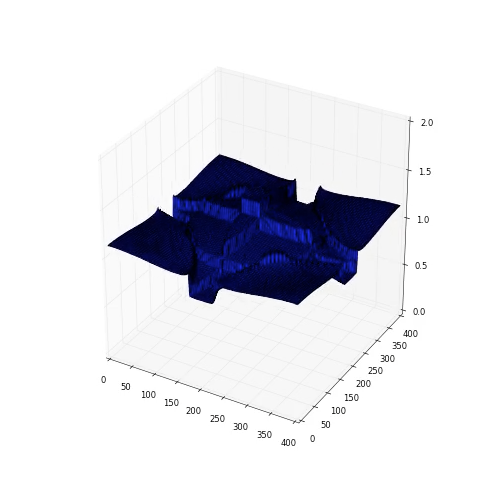
\includegraphics[width=0.6\linewidth]{shallow_wave_screenshot.png}
 \caption{Dam Break Simulation Visualization}
 \label{waterheight}
\end{figure}

\clearpage
\section{Initial C Code Profiling}

In order to determine the areas of the code to target in tuning for efficiency, we used the Intel profiling tool VTune. For a small dam break run, the slowest 18 sections of the code in terms of time are shown in Figure~\ref{v_orig}. 
 
\begin{figure}[here]
 \centering
 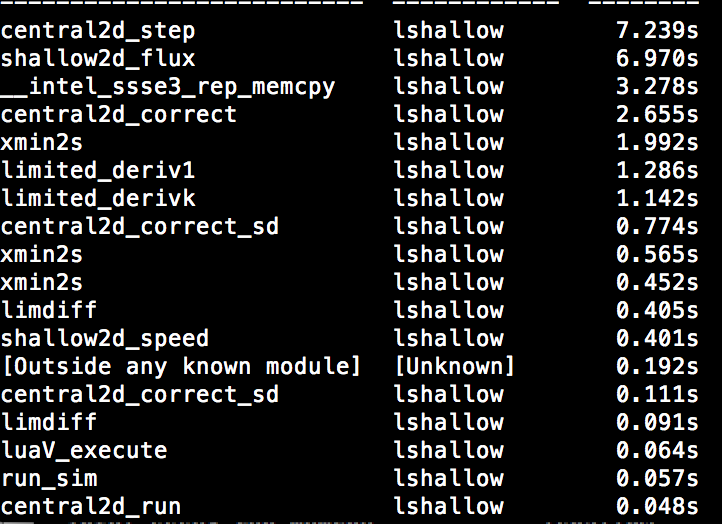
\includegraphics[width=0.4\linewidth]{VTUNE_OrigC.png}
 \caption{Vtune Output - Original Code}
 \label{v_orig}
\end{figure}

Further profiling of the slowest functions showed that the portions that contained domain computation for loops took the most time to complete. 

\section{Vectorization}
One method of speeding up the code is to use vectorization, applying operations to arrays instead of array sub elements, reducing the number of required computations. \\

To vectorize our code, we drew ideas from the vectorized C code produced by Prof. Bindel. We additionally targeted sections of our code that had to be vectorized by use of the ipo out.optreport file output after compilation, which shows the sections that have not been vectorized fully yet. Our vectorization method uses pointers to reduce overheads in manipulating the data structure. 

\section{OpenMP Parallelization}
We parallelized the code using openMP pragmas (\#pragma omp parallel) in the time advancement loop, as well as the -fopenmp flag in the compilation. Some sections, such as the new timestep computation, only needed to be performed by a single processor and so \#pargma omp single was used inside of the parallel call. At the end of each timestep, a barrier was used to allow synchronization of the processors (particularly necessary for the later domain decomposition). As all for loops were encapsulated within the timestep loop (except for the domain initialization), no additional parallel calls were needed. This parallelization was found to immensely improve the time to run the code. \\
The periodic boundary conditions were maintained from the original code, but the number of ghost cells around the domain were varied based on the number of iterations performed within a timestep. \\

\section{Domain Decomposition}
\subsection{Overview}
We decomposed the domain by creating rectangles of subdomains within the domain on which each processor solves the shallow wave equations. This was accomplished by obtaining the total number of specified threads, and breaking up the domain into that many rectangles, assuming that the domain is a square with nx=ny cells in each direction. Each thread has a section of the velocity field plus additional ghost cells copied into its own subdomain, and proceeds to solve the equations on that subdomain. After all processors have computed the new velocities for their subdomains (enforced by a barrier), the subdomain velocity fields are copied back into the overall velocity field and the timestep and periodic boundary conditions are updated for the whole domain. As before, the number of ghost cells must be varied for the number of iterations performed in a timestep in order to have enough cells to fully compute the new velocity field on the given subdomain. The number of ghost cells is set as 4*(number of subiterations), considering that the Jiang-Tadmore central difference scheme already contains an additional iteration for the predictor step.\\

\section{Processor Offloading}
Each compute node on the Totient cluster contains 24 cores. Thus, offloading to the Xeon Phi coprocessors which have 236 threads per node is desirable, particularly for large domains and numbers of desired cores. To offload to the Phis, we simply used the command: \#pragma offload target(mic:thread\_number) immediately inside the parallel section of the code after domain initialization, but prior to the time stepping section. Results comparing the C code containing the domain decomposition, vectorization, and openMP parallelization to the same code offloaded to the Xeon Phi coprocessors, and the oroginal C code, are shown in the following Results section. 

Strong scaling is viewable in the strong scaling efficiency graph - better scaling than both original and new c codes on the compute nodes. However, timings for equivalent runs take longer.

\section{Results}
Include all graphs and tables here (Being worked on!)

\section{References}

\end{document}